\documentclass[12pt, oneside]{article} 
\usepackage[a4paper]{geometry}              
\usepackage{graphicx}
\usepackage{amsmath}
\usepackage{amssymb}
\usepackage[table]{xcolor}

%SetFonts
\usepackage[T1]{fontenc}
\usepackage[bitstream-charter]{mathdesign}
%SetFonts

%define example environment 
\newcounter{examplecounter}
\newenvironment{example}%
{%
\small\begin{quote}%
\refstepcounter{examplecounter}%
\textbf{Example \arabic{examplecounter}}%
\quad%
}%
{%\schluss%
\end{quote}%
}

%define remark environment 
\newcounter{remarkcounter}
\newenvironment{remark}%
{%
\small\begin{quote}%
\refstepcounter{remarkcounter}%
\textbf{Remark \arabic{remarkcounter}}%
\quad%
}%
{%\schluss%
\end{quote}%
}

%define remark environment 
\newcounter{questioncounter}
\newenvironment{question}%
{%
\small\begin{quote}%
\refstepcounter{questioncounter}%
\textbf{Question \arabic{questioncounter}}%
\quad%
}%
{%\schluss%
\end{quote}%
}


%define important environment
\newenvironment{important}{\begin{quote}%
\textbf{Important:}%
\quad
}{%
\end{quote}%
}

\newcommand{\qed}{\nobreak \ifvmode \relax \else
      \ifdim\lastskip<1.5em \hskip-\lastskip
      \hskip1.5em plus0em minus0.5em \fi \nobreak
      \vrule height0.5em width0.5em depth0.25em\fi}

\newtheorem{theorem}{Theorem}[section]
\newtheorem{lemma}[theorem]{Lemma}
\newtheorem{proposition}[theorem]{Proposition}
\newtheorem{definition}{Definition}
\newenvironment{proof}[1][Proof]{\begin{trivlist}
\item[\hskip \labelsep {\bfseries #1}]}{\end{trivlist}}

\newcommand{\R}{\mathbb{R}}
\newcommand{\E}{\mathbb{E}}
\newcommand{\fol}{\mathcal{F}}
\newcommand{\one}{\mathbb{1}}
\newcommand{\hest}{\textsc{Hesten}}
\newcommand{\texp}{T_{\rm exp}}

\usepackage{lettrine}

\begin{document}
\noindent{\Huge \textbf\textsf{{Completing the correlation matrix in a hybrid model.}}}

\noindent \textit{by Horst K�hler, Thomas Streuer, Olaf Dreyer}

\vspace{.5cm}

\section{Introduction}

\section{The cross currency model}
To make the issues more concrete we introduce the basic cross currency model as an example. This model consists of two interest rate models and a model for the exchange rate. We will denote the base currency by $E$ and assume that we model a rate $x_E$ together with a volatility $\nu_E$. The details of the model are not important since we are only concerned about the correlation of the stochastic processes. An example of such a model would be a Heath-Jarrow€-Morton model with a stochastic volatility. The model for the foreign currency $A$ will also consist of a model for the rate $x_A$ and the volatility $\nu_A$. The remaining model will be for the exchange rate 
\begin{equation}
	X_E^A,
\end{equation}
where the lower index $E$ denotes the currency we are converting into and the upper index is the currency we are converting from. If $m_A$ is an amount in currency $A$ then
\begin{equation}
	X_E^A m_A
\end{equation}
is the corresponding amount in the currency $E$. We also assume that we are modeling the volatility $\nu_{EA}$ of the exchange rate. An example of such a model would be a Heston model \cite{heston}. Altogether we thus have these six stochastic variables:
\begin{equation}
	x_E, \nu_E, x_A, \nu_A, X_E^A, \nu_{EA}
\end{equation}
Let us denote this set of variables by $I$. For two elements $a,b\in I$ let 
\begin{equation}
	(a,b) = \langle W_a, W_b\rangle
\end{equation}
be the correlation coefficient\footnote{We introduce this non-standard notation here to improve the readability in later chapters.} for the stochastic processes of $a$ and $b$. For all $a,b\in I$ we have
\begin{align}
	(a,b) & = (b,a) \\
	(a,a) & = 1\\
	\vert(a,b)\vert & \le 1
\end{align}
In principle one could imagine that all entries of $W$ are determined in one calibration using an assortment of financial products. This is usually not what one does though because the number of parameters is too large and hence the calibration is too unstable but also because one will have already performed calibrations for the interest models themselves and thus
\begin{equation}
	(x_E, \nu_E)\text{\ and\ }(x_A, \nu_A)
\end{equation}
are already known. In addition to these two, one might decide to calibrate the coefficients
\begin{equation}
	(x_E, X_E^A),(x_E, x_A), (x_A, X_E^A)\text{, and\ } (X_E^A, \nu_{EA}).
\end{equation}
The question that arises is then how to determine the remaining coefficients (see figure \ref{fig.xccymodel}) of the correlation matrix.

\begin{figure}[hbt]
  \begin{center}
  	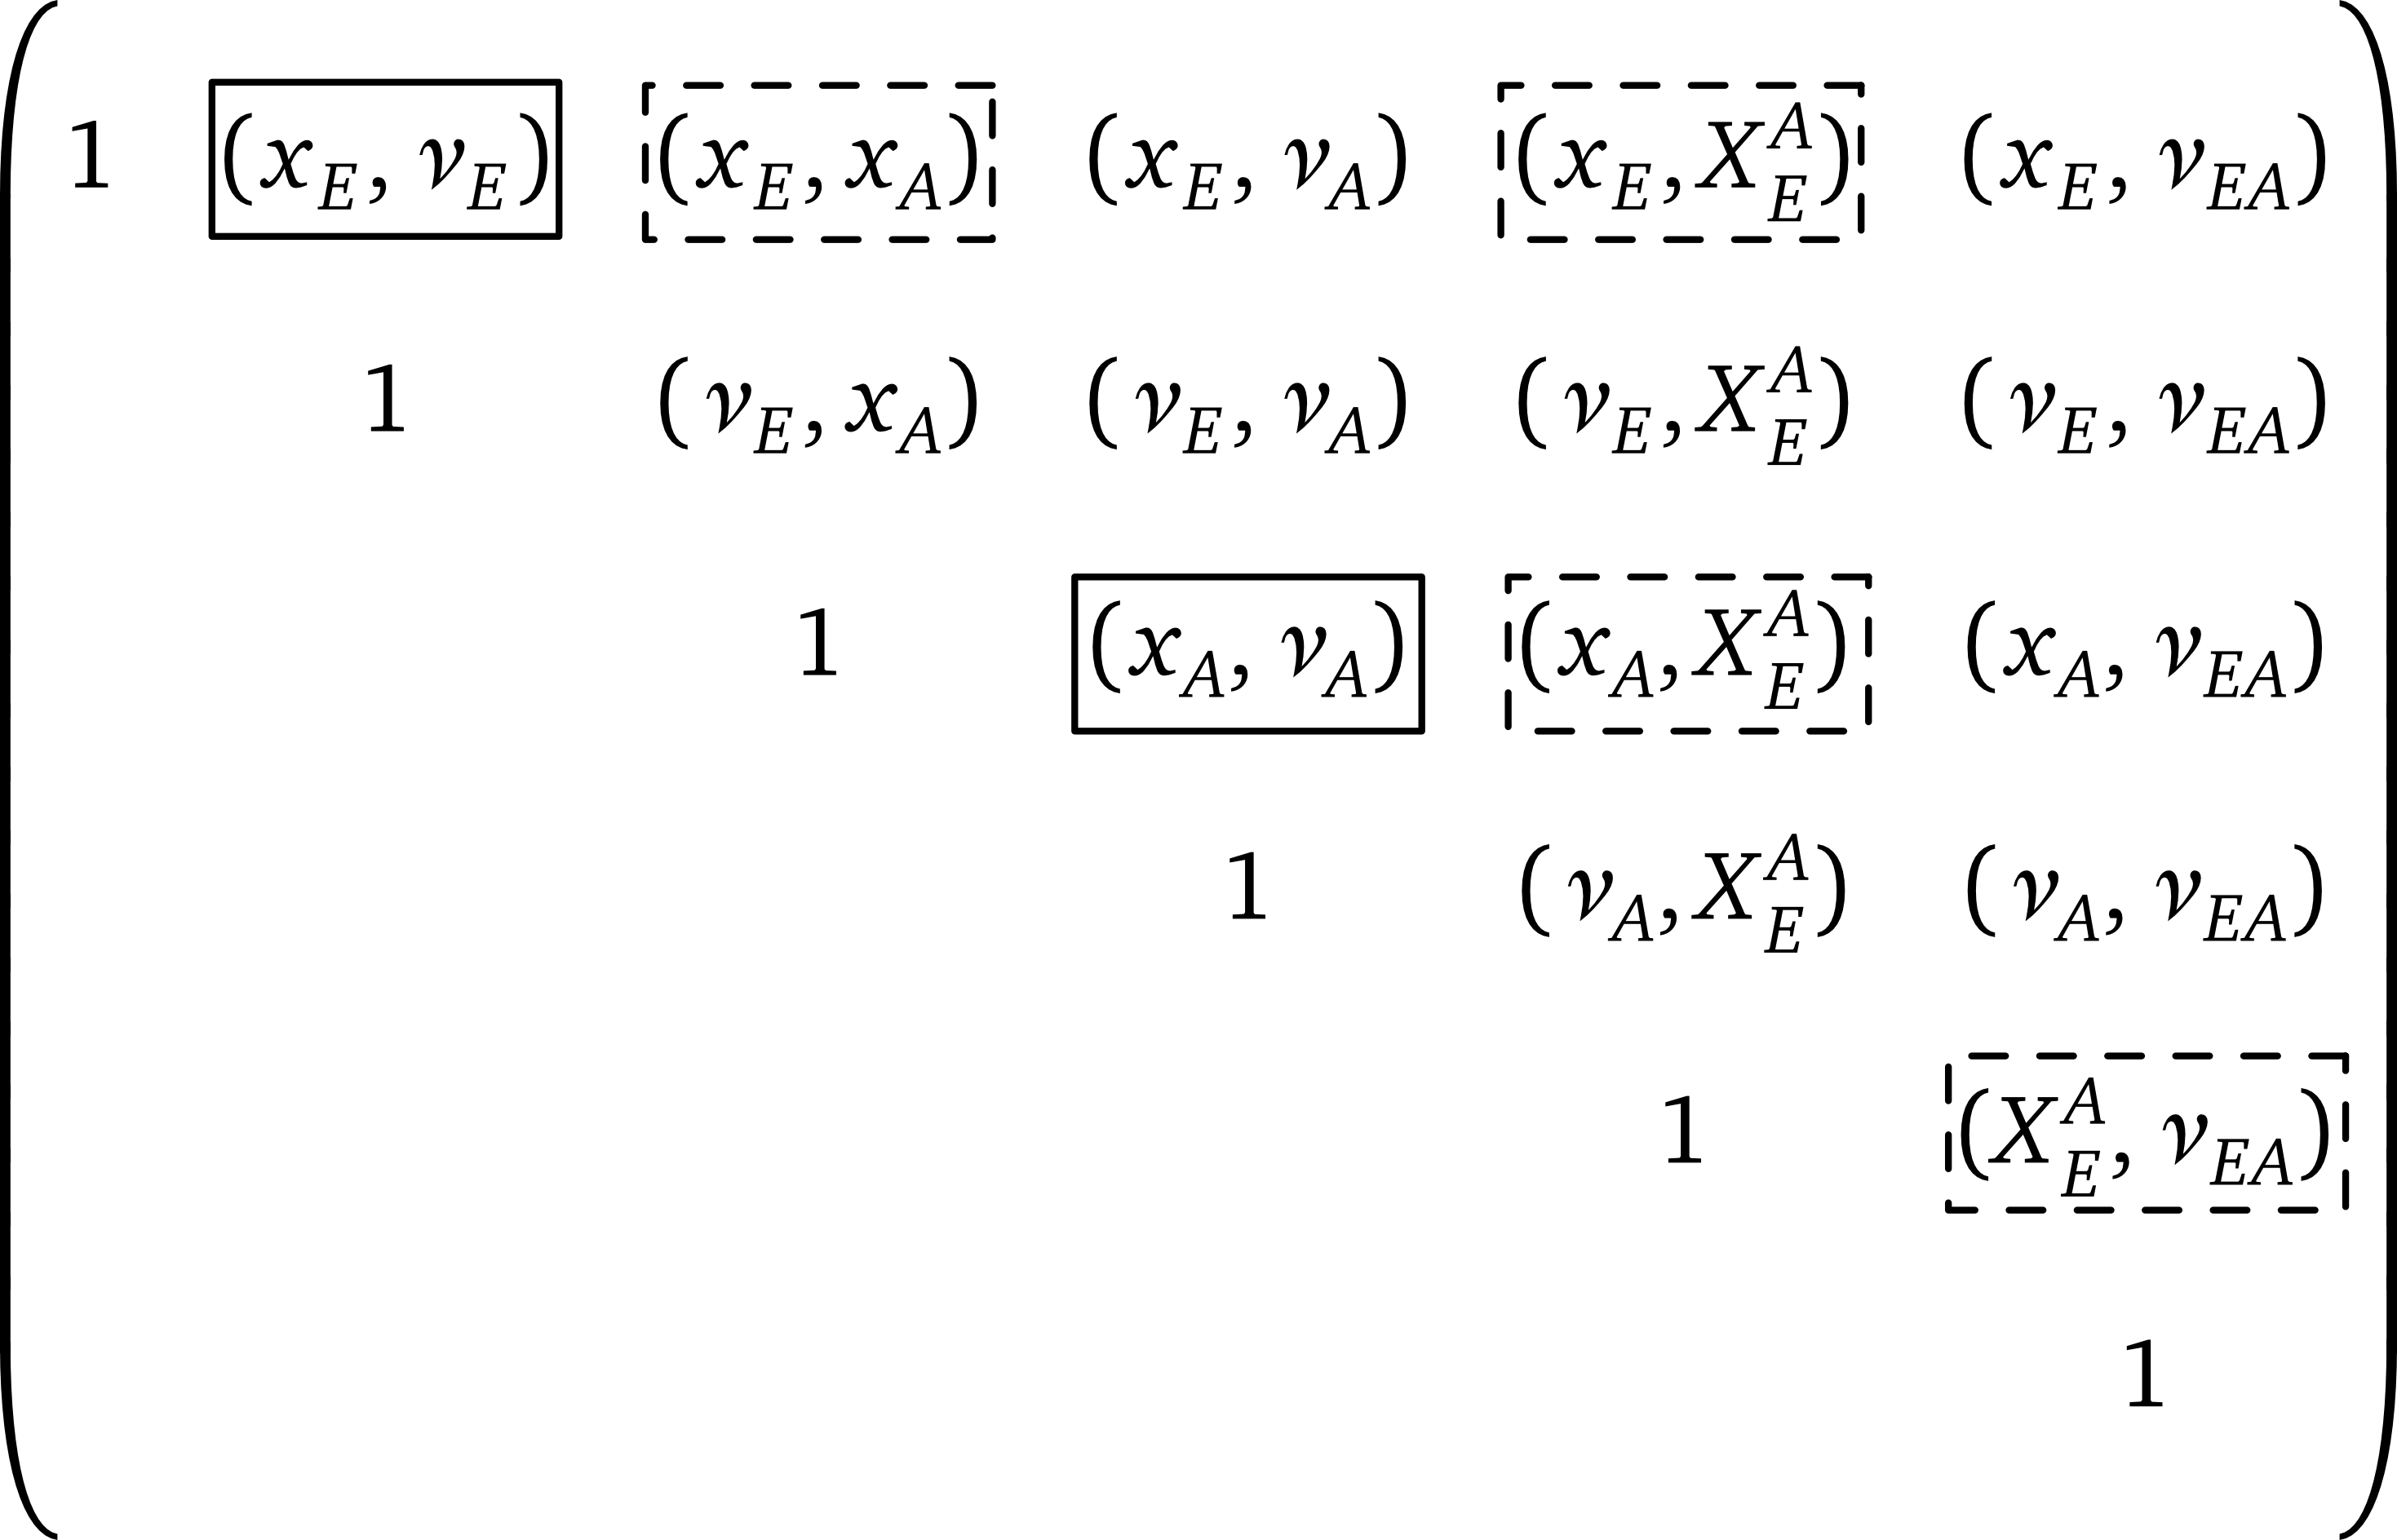
\includegraphics[width=10cm]{img/xccymodel.png}
  \end{center}
  \caption{The correlation matrix for the cross currency model. The coefficients $(x_E, \nu_E)$ and $(x_A, \nu_A)$ (the boxes with the solid lines) will be determined in two separate interest rate calibrations. The coefficients $(x_E, X_E^A)$, $(x_E, x_A)$, $(x_A, X_E^A)$, and $(X_E^A, \nu_{EA})$ (the boxes with the dashed lines) will be determined in the cross currency calibration. The question then arises what to do with he remaining coefficients?}\label{fig.xccymodel}
\end{figure}

\section{Independence, maximal determinant, and entropy}
\subsection{A simpler problem}
Before we answer the question of the last section in full generality we look at a simpler case to determine how we want to complete the matrix $M$. As in the previous section we denote by $I$ be the set of stochastic processes. For this simple case we assume that there are two sets $\alpha, \beta\subset I$ with $\alpha\cup\beta = I$ and $\alpha\cap\beta = \gamma\ne \emptyset$. For any $\delta\subset I$ we will denote by
\begin{equation}
	M[\delta]
\end{equation}
the principal submatrix of $M$ with row and column indices in $\delta$. In general we will denote for $\delta,\eta\subset I$ by 
\begin{equation}
	M[\delta,\eta]
\end{equation}
the submatrix of $M$ with row indices in $\delta$ and column indices in $\eta$. We assume that
\begin{equation}
	M[\alpha] \text{\ and\ } M[\beta] 
\end{equation}
are known. The matrix $M$ thus has the form
\begin{equation}\label{eqn.corrmatrix}
	M = \begin{pmatrix}
		C & D & W \\
		D^T & E & F \\
		W^T & F^T & G
	\end{pmatrix}.
\end{equation}
Using the notation that we have just introduced we have
\begin{align}
	M[\alpha] & = \begin{pmatrix}
		C & D  \\
		D^T & E 
	\end{pmatrix} \\
	M[\beta] & = \begin{pmatrix}
		E & F  \\
		F^T & G 
	\end{pmatrix} \\
	M[\gamma] & = E \\
	M[ \alpha-\gamma, \alpha-\gamma] & = C \\
	M[ \alpha-\gamma, \gamma] & = D \\
	M[ \alpha-\gamma, \beta-\gamma] & = W \\
	M[ \gamma, \beta-\gamma] & = F \\
	M[ \beta-\gamma, \beta-\gamma] & = F
\end{align}
The part of the matrix that we need to determine is $W$. If the overlap $E$ didn't exist we would just set $W=0$ and thus ensure that $\alpha$ and $\beta$ are independent. This is the desirable result because any other choice would assume information about the correlation between $\alpha$ and $\beta$ that we do not have. Since the overlap $E$ is present, we have to make a different choice.

\subsection{Conditioning \& Schur complement}
For $\delta\subset I$ let us assume that $M[\delta]$ is invertible (we will weaken this assumption later). Then let 
\begin{equation}
	M/M[\delta] = M[I-\delta,I-\delta] - M[I-\delta, \delta]M[\delta]^{-1}M[\delta, I-\delta]
\end{equation}
be the Schur complement\cite{hayns} (see \cite{horn} for a an overview of the properties of the Schur complement) of $M[\delta]$ in $M$. In our context the Schur complement arises naturally when we ask for the correlation matrix of a subset of the stochastic variables in $I$ conditioned on the values of the remaining variables. If the variables that we are conditioning on are in $\gamma$ then $M/M[\gamma]$ is the correlation matrix for the variables in $I-\gamma$(for a proof see \cite[chapter 8]{rao} and \cite{cottle}).

\subsection{The completion}
With the result from the last section we have a way to proceed. We can look at the correlation matrix for the elements in $I$ that we obtain when we condition on the elements in $\gamma=\alpha\cap\beta$. This matrix is given by the Schur complement
\begin{equation}
	M/M[\gamma].
\end{equation}
We can use equation (\ref{eqn.corrmatrix}) to write
\begin{align}
	M/M[\gamma] & = M/E \\
	& = \begin{pmatrix}
		C - D E^{-1} D^T & W - DE^{-1}F \\
		W^T - F^TE^{-1}D^T & G - F^TE^{-1}F
		\end{pmatrix}.
\end{align}
A special choice for $W$ now presents itself. If we choose 
\begin{equation}\label{eqn.choice}
	W = DE^{-1}F 
\end{equation}
the off-diagonal matrices vanish and the matrix becomes block-diagonal. We can even interpret the remaining blocks. We note that 
\begin{align}
	M[\alpha]/M[\gamma] & = C - D E^{-1} D^T \\
	M[\beta]/M[\gamma] & = G - F^TE^{-1}F.
\end{align}
Again, using the result from the previous section, we see that the remaining blocks give the correlation matrix for $\alpha$ and $\beta$ respectively, when we condition on $\gamma$. The block-diagonal form in equation (\ref{eqn.choice}) says that the variables $\alpha$ conditioned on $\gamma$ are independent from the variables $\beta$ conditioned on $\gamma$. If $f$ is the corresponding density function we have
\begin{equation}
	f(x_{I-\gamma} \vert \gamma ) = f(x_{\alpha-\gamma} \vert \gamma )f(x_{\beta-\gamma} \vert \gamma ).
\end{equation}
Given that $\gamma$ is shared by both $\alpha$ and $\beta$ this is the most independence we can hope for. 

\subsection{Maximal determinant}
Another way to characterize the choice of $W$ in equation (\ref{eqn.choice}) is by looking at the determinant of $M$. In general we have 
\begin{align}
	\det(M) & = \det(M[\gamma]) \det(M/M[\gamma]) \\
	& \le \det(M[\gamma]) \det(M[\alpha]/M[\gamma]) \det(M[\beta/M[\gamma]),\label{eqn.upperbound}
\end{align}
(see \cite{horn} for the first equality), where we have used the Fischer inequality in the second line. With $W$ as in equation (\ref{eqn.choice}) the Schur complement $M/M[\gamma]$ becomes block-diagonal and we obtain
\begin{equation}
	\det(M) = \det(M[\gamma]) \det(M[\alpha]/M[\gamma]) \det(M[\beta/M[\gamma]).
\end{equation}
The determinant thus reaches the upper bound of equation (\ref{eqn.upperbound}). Choosing $W$ as in equation (\ref{eqn.choice}) we thus maximize the determinant of $M$. 

\subsection{Zeroes \& the inverse matrix}
A remarkable formula due to Babachiewicz \cite{horn} expresses the inverse of a matrix in terms of the Schur complement. For a matrix
\begin{equation}
	\Sigma = \begin{pmatrix}
		\Sigma_{11} & \Sigma_{12} \\ 
		\Sigma_{21} & \Sigma_{22}
	\end{pmatrix}
\end{equation}
we have
\begin{equation}
	\Sigma^{-1} = \begin{pmatrix}
		\Sigma_{11}^{-1} + \Sigma_{11}^{-1}\Sigma_{12}(\Sigma/\Sigma_{11})^{-1}\Sigma_{21}\Sigma_{11}^{-1} &-\Sigma_{11}^{-1} \Sigma_{12} (\Sigma/\Sigma_{11})^{-1} \\ 
		-(\Sigma/\Sigma_{11})^{-1}\Sigma_{21}\Sigma_{11}^{-1} & (\Sigma/\Sigma_{11})^{-1}
	\end{pmatrix}.
\end{equation}
This formula has the remarkable property that only the inverses 
\begin{equation}
	\Sigma_{11}^{-1} \text{\ and\ } (\Sigma/\Sigma_{11})^{-1}
\end{equation}
appear in it. With our choice of $W$ in equation (\ref{eqn.choice}) the Schur complement $M/E$ is block diagonal. This means that also its inverse is block diagonal. Indeed, we have
\begin{equation}
	(M/E)^{-1} = \begin{pmatrix}
		(M[\alpha]/E)^{-1} & 0 \\
		0 & (M[\beta]/E)^{-1}
	\end{pmatrix}.
\end{equation}
This allows us to write the inverse of $M$ explicitly:
\begin{equation}
	M^{-1} = \begin{pmatrix}
		(M[\alpha]/E)^{-1} & -(M[\alpha]/E)^{-1} D E^{-1} & 0 \\
		- E^{-1} D^T (M[\alpha]/E)^{-1} & \Xi & - E^{-1} F (M[\beta]/E)^{-1} \\
		0 & - (M[\beta]/E)^{-1} F^T E^{-1} & (M[\beta]/E)^{-1}
	\end{pmatrix},
\end{equation}
with
\begin{equation}
	\Xi = E^{-1} + E^{-1}\left(D^T(M[\alpha]/E)^{-1}D + F (M[\beta]/E)^{-1} F^T\right)E^{-1}.
\end{equation}
We see that the inverse of $M$ has zeroes in exactly those places where the undetermined matrix $W$ used to be.

\subsection{Entropy}
The determinant of $M$ is directly related to the entropy of the distribution that is described by $M$:
\begin{equation}
	S = \frac{1}{2}\big(\log(\det(M)) + n \log(2\pi) + n\big)
\end{equation}
Because we are maximizing the determinant we are also maximizing the entropy. 

\subsection{The semidefinite case}

\section{The completion procedure}

\section{The general hybrid model}

\begin{thebibliography}{MM}
	\bibitem{heston} Steven L. Heston, A Closed-Form Solution for Options with Stochastic Volatility with Applications to Bond and Currency Options, The Review of Financial Studies, \textbf{6}(2), April 1993, 327--343.
	\bibitem{hayns} Emilie Virginia Haynsworth, Determination of the inertia of a partitioned Hermitian matrix,  Linear  Algebra and its Applications \textbf{1}, 1968, 73--81. 
	\bibitem{horn} Roger A. Horn, Basic  Properties  of  the  Schur  Complement. In Fuzhen Zhang (Ed.) The Schur complement and its application (17--46). Springer, 2005.
	\bibitem{rao} C. Radharkishna Rao, Linear Statistical Inference and its Applications, 2nd edition, John Wiley \& Sons, Inc, 2002.
	\bibitem{cottle} Richard W. Cottle, Manifestations of the Schur complement, Linear Algebra and its Applications \textbf{8}, 1974, 189--211. 
\end{thebibliography}


\end{document}